%%
%% This is file `sample-authordraft.tex',
%% generated with the docstrip utility.
%%
%% The original source files were:
%%
%% samples.dtx  (with options: `authordraft')
%% 
%% IMPORTANT NOTICE:
%% 
%% For the copyright see the source file.
%% 
%% Any modified versions of this file must be renamed
%% with new filenames distinct from sample-authordraft.tex.
%% 
%% For distribution of the original source see the terms
%% for copying and modification in the file samples.dtx.
%% 
%% This generated file may be distributed as long as the
%% original source files, as listed above, are part of the
%% same distribution. (The sources need not necessarily be
%% in the same archive or directory.)
%%
%% Commands for TeXCount
%TC:macro \cite [option:text,text]
%TC:macro \citep [option:text,text]
%TC:macro \citet [option:text,text]
%TC:envir table 0 1
%TC:envir table* 0 1
%TC:envir tabular [ignore] word
%TC:envir displaymath 0 word
%TC:envir math 0 word
%TC:envir comment 0 0
%%
%%
%% The first command in your LaTeX source must be the \documentclass command.
\DocumentMetadata{}
\documentclass[sigconf,nonacm]{acmart}
%% NOTE that a single column version may required for 
%% submission and peer review. This can be done by changing
%% the \doucmentclass[...]{acmart} in this template to 
%% \documentclass[manuscript,screen]{acmart}
%% 
%% To ensure 100% compatibility, please check the white list of
%% approved LaTeX packages to be used with the Master Article Template at
%% https://www.acm.org/publications/taps/whitelist-of-latex-packages 
%% before creating your document. The white list page provides 
%% information on how to submit additional LaTeX packages for 
%% review and adoption.
%% Fonts used in the template cannot be substituted; margin 
%% adjustments are not allowed.
%%
%% \BibTeX command to typeset BibTeX logo in the docs
\AtBeginDocument{%
  \providecommand\BibTeX{{%
    \normalfont B\kern-0.5em{\scshape i\kern-0.25em b}\kern-0.8em\TeX}}}

%% Rights management information.  This information is sent to you
%% when you complete the rights form.  These commands have SAMPLE
%% values in them; it is your responsibility as an author to replace
%% the commands and values with those provided to you when you
%% complete the rights form.
\setcopyright{acmcopyright}
\copyrightyear{2026}
\acmYear{2026}
\acmDOI{XXXXXXX.XXXXXXX}

%% These commands are for a PROCEEDINGS abstract or paper.
\acmConference[Conference acronym 'XX]{Make sure to enter the correct
  conference title from your rights confirmation emai}{June 03--05,
  2018}{Woodstock, NY}
%
%  Uncomment \acmBooktitle if th title of the proceedings is different
%  from ``Proceedings of ...''!
%
%\acmBooktitle{Woodstock '18: ACM Symposium on Neural Gaze Detection,
%  June 03--05, 2018, Woodstock, NY} 
\acmPrice{15.00}
\acmISBN{978-1-4503-XXXX-X/18/06}


%%
%% Submission ID.
%% Use this when submitting an article to a sponsored event. You'll
%% receive a unique submission ID from the organizers
%% of the event, and this ID should be used as the parameter to this command.
%%\acmSubmissionID{123-A56-BU3}

%%
%% For managing citations, it is recommended to use bibliography
%% files in BibTeX format.
%%
%% You can then either use BibTeX with the ACM-Reference-Format style,
%% or BibLaTeX with the acmnumeric or acmauthoryear sytles, that include
%% support for advanced citation of software artefact from the
%% biblatex-software package, also separately available on CTAN.
%%
%% Look at the sample-*-biblatex.tex files for templates showcasing
%% the biblatex styles.
%%

%%
%% For managing citations, it is recommended to use bibliography
%% files in BibTeX format.
%%
%% You can then either use BibTeX with the ACM-Reference-Format style,
%% or BibLaTeX with the acmnumeric or acmauthoryear sytles, that include
%% support for advanced citation of software artefact from the
%% biblatex-software package, also separately available on CTAN.
%%
%% Look at the sample-*-biblatex.tex files for templates showcasing
%% the biblatex styles.
%%

%%
%% The majority of ACM publications use numbered citations and
%% references.  The command \citestyle{authoryear} switches to the
%% "author year" style.
%%
%% If you are preparing content for an event
%% sponsored by ACM SIGGRAPH, you must use the "author year" style of
%% citations and references.
%% Uncommenting
%% the next command will enable that style.
%%\citestyle{acmauthoryear}

%%
%% end of the preamble, start of the body of the document source.

\begin{document}

%%
%% The "title" command has an optional parameter,
%% allowing the author to define a "short title" to be used in page headers.
\title{P2P File-Sharing Application using Go, Java, and Python}
\subtitle{\href{https://github.com/dobaj/cisc468-final-project}{https://github.com/dobaj/cisc468-final-project}}

%%
%% The "author" command and its associated commands are used to define
%% the authors and their affiliations.
%% Of note is the shared affiliation of the first two authors, and the
%% "authornote" and "authornotemark" commands
%% used to denote shared contribution to the research.
\author{Alice Fraimovich (20356347, 21amf28@queensu.ca)}
\author{Matt Dobaj (20350312, 21mtd4@queensu.ca)}
\author{Nicholas Wang (20364023, 22nw@queensu.ca)}


%%
%% By default, the full list of authors will be used in the page
%% headers. Often, this list is too long, and will overlap
%% other information printed in the page headers. This command allows
%% the author to define a more concise list
%% of authors' names for this purpose.
\renewcommand{\shortauthors}{Dobaj, Fraimovich, and Wang}

%%
%% The abstract is a short summary of the work to be presented in the
%% article.
\begin{abstract}
This report analyzes the structure and implementation of our peer-to-peer file-sharing application, including detailing the system overview and architecture, protocol design and communication flow, algorithms and encryption scheme utilized and message format and types. We outline the process of designing a secure file-sharing system that guarantees integrity, and explain our reasoning behind each of the design choices made. Finally, we discuss error handling and edge cases, any problems we had run into and libraries used.  In the first section, we demonstrate our planning through outlining our objectives for our application, and any sources we used in our research for this project. Our next section delves into our precise architecture and overview of the system(s) we implemented. Lastly, we lay out our process for testing and implementing the final aspects of the file-sharing application, including error-handling and edge cases, along with detailing all libraries used.
\end{abstract}

%%
%% The code below is generated by the tool at http://dl.acm.org/ccs.cfm.
%% Please copy and paste the code instead of the example below.
%%
%\begin{CCSXML}
%<ccs2012>
% <concept>
  %<concept_id>00000000.0000000.0000000</concept_id>
  %<concept_desc>Do Not Use This Code, Generate the Correct Terms for Your Paper</concept_desc>
  %<concept_significance>500</concept_significance>
 %</concept>
 %<concept>
%  <concept_id>00000000.00000000.00000000</concept_id>
  %<concept_desc>Do Not Use This Code, Generate the Correct Terms for Your Paper</concept_desc>
  %<concept_significance>300</concept_significance>
 %</concept>
 %<concept>
%  <concept_id>00000000.00000000.00000000</concept_id>
  %<concept_desc>Do Not Use This Code, Generate the Correct Terms for Your Paper</concept_desc>
  %<concept_significance>100</concept_significance>
 %</concept>
 %<concept>
%  <concept_id>00000000.00000000.00000000</concept_id>
  %<concept_desc>Do Not Use This Code, Generate the Correct Terms for Your Paper</concept_desc>
  %<concept_significance>100</concept_significance>
 %</concept>
%</ccs2012>
%\end{CCSXML}

%\ccsdesc[500]{Do Not Use This Code~Generate the Correct Terms for Your Paper}
%\ccsdesc[300]{Do Not Use This Code~Generate the Correct Terms for Your Paper}
%\ccsdesc{Do Not Use This Code~Generate the Correct Terms for Your Paper}
%\ccsdesc[100]{Do Not Use This Code~Generate the Correct Terms for Your Paper}

%%
%% Keywords. The author(s) should pick words that accurately describe
%% the work being presented. Separate the keywords with commas.
%\keywords{Do, Not, Us, This, Code, Put, the, Correct, Terms, for, Your, Paper}

% \received{20 February 2007}
% \received[revised]{12 March 2009}
% \received[accepted]{5 June 2009}

%%
%% This command processes the author and affiliation and title
%% information and builds the first part of the formatted document.
\maketitle

\section{Introduction}
A P2P file-sharing application enables users to send and receive files directly between peers. For our application, these users must share a local network in order to send and receive files, and users can use clients written in Python, Java, and Go. These clients must use a standardized communication protocol that supports well-defined cryptographic primitives, and must guarantee confidentiality, integrity, and message authentication. 

A key challenge in this environment is interoperability, as although each client is implemented in a different language and utilizes different libraries, they are still expected to discover one another, ensure identities are authenticated, and exchange files securely. In an effort to address these expectations, our system defines a shared wire protocol based on JSON messages and common cryptographic operations.

\subsection{Project Objectives}
When creating our secure P2P file-sharing application, we first needed to outline our primary objectives. These objectives were to ensure the application supported peer discovery on mDNS, mutual authentication of contacts, requesting of and sending files to and from other peers on the shared network, listing available files, and retrieving files from offline users. Regarding encryption, we also required confidentiality and the ability to migrate to a new key. Ensuring the integrity of all transferred files was also vital to prevent unauthorized tampering during transit. Beyond these core features, we prioritized the implementation of perfect forward secrecy, as it ensures that “the compromise of long-term keys does not allow an attacker to obtain past session keys.”\cite{Paar:2024} On the client side, we focused on secure local storage in an effort to protect more sensitive data from being accessed even if the physical device was stolen. We also integrated comprehensive error handling to provide users with clear feedback regarding delivery failures or failed security checks, such as detected file tampering. We met these objectives by selecting libraries and security parameters that would aid us in meeting our security objectives, all while further maintaining a functional peer-to-peer environment.

\section{System Overview and Architecture}
The architecture of our application is designed as a decentralized peer-to-peer system that uses mDNS to facilitate secure communication, and more importantly, secure file transfer between clients written in Python, Java, and Go. The system utilizes a multi-layered approach to peer interaction, and it begins with discovery via mDNS, prompting clients to broadcast their presence on a local network. Clients can automatically find available peers and mDNS reliably retrieves their name and IP/port. Once a peer is selected by one client, they can establish a TCP connection to begin communication. After this TCP connection is established, the two peers perform an authentication handshake. During this handshake, each side exchanges a long-term Ed25519 identity public key and a fresh X25519 ephemeral public key. The handshake transcript is signed with the Ed25519 private key and verified by the other side before communication continues. Using the exchanged X25519 ephemeral public keys, both peers compute a shared secret, which is then passed through HKDF-SHA256 to derive the symmetric session key used for the rest of the session. This session key is then used with AES-GCM to encrypt and authenticate all subsequent communication between the two peers. The presented identity key is then checked against the local trust store. If the key is already trusted, the session continues. If it is unknown, the user is shown the fingerprint and asked whether to trust it. If it conflicts with a previously trusted key, the connection is rejected. Following successful verification of the peer’s identity, secure communication continues for file listing, requests, and retrieval of files from offline peers.

In regards to file retrieval and requesting files from an offline user, once a secure session has been established, a client can request a list of files available from another peer and then request a specific file for transfer. File metadata, which includes hashes and information of ownership, is used to verify integrity and track the original source of the selected file. In this way, the design supports retrieval from an offline user through cached file records. If a user who originally owned a file is no longer connected, another peer that had previously received and stored that file can provide it to the other user, as long as the cached metadata matches the original owner and the file hash verifies correctly. Thus, the system is able to support more flexible peer-to-peer file availability.

Files are also securely stored on the user’s device using AES-GCM and a key that is derived from the user’s input passphrase using PBDKF. Files that are received and placed in this encrypted store can be decrypted and written to the disk unencrypted to share with others.

The application also supports key migration to allow a user to continue secure file transfer after a public-private identity key is compromised. A user can generate a new public-private identity key and send a message to its peers with its new key, the new key signed with its old key, and the old key is signed with its new key, to prove that the user has access to both pairs. This does assume, however, that the user is able to change keys before the attacker does.

\subsection{Protocol Design and Communication Flow Diagram}
\begin{figure}[h]
  \centering
  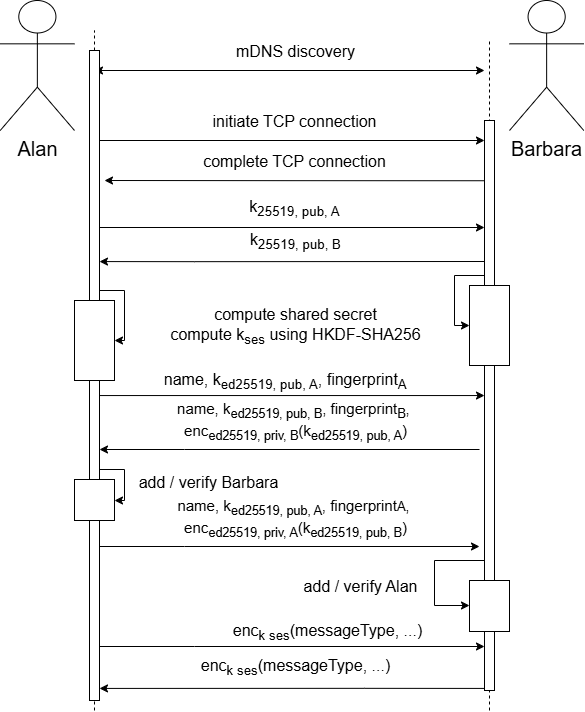
\includegraphics[width=\linewidth]{authenticationDiagram.png}
  \caption{Diagram depicting the handshake protocol.}
  \Description{Diagram depicting the handshake protocol.}
\end{figure}
Messages are encoded as JSON and framed with a 4-byte length prefix so each client can reliably distinguish message boundaries on the stream. 

As previously mentioned, a session key exchange is first performed before each user’s identity is exchanged. In our codebase, we only share the public key for each user back and forth in order to identify each user, but given more time we would modify our code bases to sign every peer’s fingerprints as shown, or more optimally, sign a challenge nonce to prove that a user has access to both their private and public key. This extension would be implemented to prevent replay attacks.

\subsection{Cryptography and Security Design}

\subsubsection{Key Exchange and Authentication}

We made the decision to use Ed25519 for long-term identity keys and digital signatures. Ed25519 is a public-key signature scheme based on elliptic curve cryptography, and it is reliable as it is a secure and efficient method for authentication. It enables each client to maintain a persistent identity key pair, where the public key can be used to generate a fingerprint that identifies the peer. Thus, Ed25519 allows clients to verify that the other party is the expected peer.

Ephemeral key exchange for session keys is performed using X25519 elliptical curve Diffie-Hellman exchange because it allows two peers to securely establish a shared secret over an untrusted network without sending the secret itself. X25519 is well suited for this purpose because of its efficiency, it is widely used, and designed specifically for secure key agreement. Its usage also guarantees that each session generates a fresh shared secret, thus also improving security.

\subsubsection{Key Derivation}

Session keys are derived from the X25519 shared secret using HKDF-SHA256 because the raw shared secret produced by Diffie-Hellman is not intended to be used as an encryption key directly, and therefore HKDF provides a secure way to extract and expand that shared secret into a strong key that is suitable for symmetric encryption. Using SHA-256 within HKDF helps ensure that the derived session keys are secure against attacks. Ed25519 and X25519 use 256-bit keys, making them efficient while still providing strong protection against malicious intent.

\subsubsection{File Message Format}

When sending files back and forth between clients, they are sent along with the file owner’s name, the size of the file, the file’s SHA256 hash, a signature of the previously mentioned elements, and the owner’s public key. The signature of the vital elements is checked with the file owner’s public key to verify that they are unmodified. The hash is used to verify that the file is unmodified.

\section{Error Handling and Edge Cases}
Incoming files have their signature verified using the file owner’s public key and their hash checked to prevent in-transit modification. If these modifications are detected or other errors occur, then the user is notified and the files are not saved, but the clients continue their connection. If errors are raised when generating keys or when traversing directories, the clients exit as these errors impede the app usage. 

\subsection{Libraries}
Across all clients in our project, the main external dependencies support cryptography and local peer discovery. The Python client makes use of cryptography\cite{PyCA01} and zeroconf\cite{Pzconf01}, the Java client utilizes Bouncy Castle\cite{BouncyCastle01}, Gson\cite{Gson01}, and JmDNS\cite{JmDNS01}, and the Go client primarily uses the standard crypto library with libraries for PKCS\#8 key handling\cite{Youmark01} and mDNS peer discovery\cite{Grandcat01}. These libraries were chosen because they are able to provide very stable, well-supported implementations of the primary features required for our P2P system.  Cryptographic libraries securely handle identity keys, signatures, key exchange, and encryption without implementing algorithms from scratch. Our decision to rely on the cryptographic library is based around the following core principle when designing a secure system: “Never ever develop your own cryptographic algorithm unless you have a team of experienced cryptanalysts checking your design.”\cite{Paar:2024}

\section{Limitations}
There were several limitations encountered in the implementation of our P2P file-sharing application. One issue we identified was that the clients should send a nonce-based challenge when verifying to prove that the user being interacted with actually has the private key corresponding to the public key they present, but this is tested when sending files. This issue was discovered late into development and was not during protocol design, and so it is not addressed in the codebase. Another limitation is that  trust on first use assumes there is an out of channel means of verifying that the user connecting is not malicious. File transfer also has a crucial limitation. File chunking was not fully working, so the system can only send files smaller than 10MB, which is the maximum message size supported by the protocol.

Another significant limitation was discovered in our key migration process. Due to the fact that a user’s key is changed by proving that they have access to their old key, an attacker that has knowledge of a user’s old private-public key pair can migrate to a new key themselves before the legitimate user is able to . This would be a key pair that the legitimate user does not know. A comparable analogy would be an attacker altering a user’s password on a website following their discovery of the user’s password. This would happen before the user is able to change the password themselves. This limitation is unavoidable given our design, as users only trust other users based on their public key fingerprints.

\section{Lessons Learned}
With a project of this scope, we realized that working slowly and methodically was vital to success. Working in stages is instrumental when it comes to making certain that all components function properly. In order to make bugs easier to find, we should have made a minimum viable product by first ensuring all clients can communicate unencrypted and then verifying that they can authenticate properly with each other. We could have then moved on to making sure that all communication was encrypted, and finally adding all additional features after the previous steps were completed. Having checkpoints would have greatly reduced and distributed our workload more effectively over the course of the semester. Having regular testing at each step would also have helped improve the robustness of our clients.  

We also learned that having a rigorous agreed upon protocol is the best foundation for a cryptographically secure peer-to-peer file sharing application. There were some aforementioned issues with our protocol, which we could have found if we had a more detailed planning stage that could have made use of diagrams, for example. Comparing these diagrams with those found in the class slides or the textbook would quickly have shown gaps in our security. 

One final way we could have improved our collaboration would have been to initiate more frequent group coding and testing sessions.   We had organized check-in meetings on a weekly basis, but working through different stages of the project together would have alerted us to shared issues earlier, giving us time to fix them quickly. 

Our testing approach followed a similar, infrequent pattern and unfortunately would result in multiple bugs that needed to be resolved each meeting. Having more frequent testing meetings would have allowed us to test every step of the project individually, ensuring that we had stayed on track and avoided any major issues from piling up. 


\section{Conclusion}
Our peer-to-peer file sharing application was instrumental in helping us learn how to tackle unexpected issues in our code, working as a team, and learning the basics of cryptography. We established a shared protocol based around stronger ecliptic based versions of the methods for key derivation and signature functions in class, and were able to successfully transfer files to and from different clients. It was a necessary challenge that pushed us to our limits and taught us that oftentimes things do not go as planned. We also discovered some limitations and issues with our protocol which could be exploited by an attacker, which was to be expected. As the saying goes, never roll your own crypto. 
%%
%% The next two lines define the bibliography style to be used, and
%% the bibliography file.
\bibliographystyle{ACM-Reference-Format}
\bibliography{report-base}

\end{document}
\endinput
%%
%% End of file `sample-authordraft.tex'.
